\section{Deploying \toolname}
\label{sec:deployment}

We set out to answer the following questions:

\begin{itemize}
\item \textbf{Q1}: What kinds of mistakes do users make in interactive proofs, and how do they fix them? (Section~\ref{sec:q1})
\item \textbf{Q2}: What kinds of changes to programs and specifications do users
make often, and do those changes reveal patterns amenable to automation? (Section~\ref{sec:q2})
\end{itemize}
To answer these questions, we recruited 12 proof
engineers to install \toolname and use Coq normally for
a month (Section~\ref{sec:recruiting}).
We received a month's worth of data containing granular detail on
Coq development for 8 of 12 of those users
(Section~\ref{sec:collection}).
After a month, we shut down the server, closed the study,
and visualized and analyzed the data (Section~\ref{sec:analysis}).

\subsection{Recruiting}
\label{sec:recruiting}

We recruited proof engineers by distributing a promotional video
and study description.
\iffalse
 to the \lstinline{coq-club} email list, on Twitter,
and directly to professors at universities with many Coq users.
\fi
All potential users went through a screening process, ensuring that they are
at least 18 years old, fluent in English, and have at least a year of experience using Coq.
Upon installation of the plugin, users filled out a consent form.
Users then filled out a questionnaire about Coq background and usage,
the results of which are in Figure~\ref{tab:users}.

All users reported more than 2 years of experience;
7 reported more than 4.
Self-assessed expertise was evenly distributed between intermediate,
knowledgeable, and expert; no beginners or novices participated.
4 users reported that they use Coq for writing mathematical proofs,
while the other 8 reported that they use Coq for verifying software.
7 users said that they use Coq every day, 2 a few times per week,
and 3 a few times per month.
10 users reported using Proof General, while 1 user reported using
\lstinline{coqtop}, and 1 user reported using a custom UI.
4 users installed the plugin with the master branch of Coq,
while 4 users used Coq 8.10, 2 users used Coq 8.9,
and 2 users used Coq 8.8.

\subsection{Collection}
\label{sec:collection}

The study period lasted one month, during which users agreed to develop
Coq code with the plugin enabled whenever possible, or otherwise let us know
why this was not possible.
All of the data collected within this time period
has been made publicly available with the consent of the users.\footnote{\url{http://github.com/uwplse/analytics-data}}

Figure~\ref{tab:sessions} shows the number of sessions by user.
Every time the plugin was loaded, either inside of a compiled file
or inside of a file open in a UI, this began a new session.
For both Q1 and Q2, our analyses looked for changes only within
sessions that involved some combination of failure
and stepping up and then back down in a UI;
we call these \textit{interactive sessions}.

We marked a session as interactive if it contained at least
one cancellation followed by other changes in
state. This did not capture any compilation passes
because Coq disallows cancellations outside of interactive mode.
For example, User 3 logged 11495 total sessions, only 101
of which were interactive. 
The remainder of User 3's sessions were, for the most part,
compilation passes over large sets of dependencies (one session per dependency).
In total, across all users, there were 362 interactive sessions.

Within these interactive sessions, the analysis for Q1 looked for 
fixes to failing tactics only inside of spans of time spent 
\emph{inside proofs} that involved some combination of failure and
stepping up and then back down in a UI;
we call these \textit{interactive proof subsessions}.
There could be zero, one, or multiple of these within an interactive session.
We detected these similarly to how we detected
interactive sessions.
There were 279 interactive proof subsessions.

\toolname logged interactive sessions for only 8 of the 12 users.
Section~\ref{sec:discussion} discusses possible causes of, implications of,
and remedies for this.
%We speculate as to why, consider the implications,
%and discuss how to reach more users in Section~\ref{sec:discussion}.

\subsection{Analysis}
\label{sec:analysis}

Once we had collected this data, we analyzed it to answer Q1 and Q2.
To answer these questions, we developed a small Python
codebase to analyze the data.
The scripts used information about cancellations
to build visualizations to aid in analysis.
For Q1, we built this cancellation information into a search tree for
each proof, and produced visualizations of each tree
(see \Cref{fig:search-tree}).
For Q2, we used this cancellation
information to reconstruct a sequence of diffs, and used Git tooling
to manually inspect these diffs (see \Cref{fig:ex-diff}).

The scripts, visualizations, and results for Q1 and Q2 can
be found alongside the data in the public data repository. 

\section{Q1: Mistakes In and Fixes to Proofs}
\label{sec:q1}

Q1 asked what mistakes proof engineers
make in proofs, and how they fix those mistakes.
This data may inform the development of tools
that help users write proofs
by suggesting next steps and changes to existing tactics.

\paragraph{A1}
We found the following:

\begin{enumerate}
\item Most interactive proof subsessions ended
  in the user stepping up to an earlier definition.
This shows that writing definitions and proofs about those definitions was
usually a feedback loop. (Section~\ref{sec:feedback})
\item Within proofs, application of lemmas
was the main driver of proving. (Section~\ref{sec:tactics})
\item Within proofs, over half of fixes to tactic mistakes
fixed either an improper argument or wrong sequencing structure.
(Section~\ref{sec:fixes})
\end{enumerate}

\paragraph{Methodology}
Our analysis for Q1 looked within the 279 interactive proof subsessions.
We first counted the number of times each tactic was used, the number
of times it was stepped above, and the number of times its invocation
caused an error. Then, we constructed a search tree using the
cancellation structure, and for any state which had multiple out edges
(a proof state where multiple tactics were tried), we compared the
cancelled attempts to the final tactic used.

\subsection{Fixing Proofs by Fixing Definitions}
\label{sec:feedback}

Of the 279 interactive proof subsessions, 209 (over 75\%) began a proof,
only to step above the entire proof attempt and
return to make changes to earlier definitions or commands, for example
to change a specification to make the proof possible.
This suggests that tools that attempt to provide next steps to users writing proof
may also benefit from suggesting possible fixes to definitions used in the proof.
% ,as the proof often cannot be completed without first changing definitions.
% ^ Talia: We can't claim "often cannot," but I think it's OK to omit
\begin{displayquote}
  \textbf{Takeaway:}
  It may be beneficial to combine machine learning tools
  that automatically complete or suggest hints for
  proofs~\cite{proverbot9001, Komendantskaya2012, Nagashima2018, Gauthier2017b,
    Yang2019}
  with tools for repairing definitions~\cite{Ringer2018, robert2018}.
\end{displayquote}

We considered only the remaining 70 successful interactive proof subsessions
(made up of 1085 tactic invocations)
for the sake of analyzing behavior \textit{within} proofs that
ended in a successful proof.
The analysis for Q2 (Section~\ref{sec:q2}) reveals more about
how specifications and programs changed.

\begin{figure}
\small
  \begin{tabular}{|l|c|c|c|}
    \hline
    \textbf{Tactic} & \textbf{Used} & \textbf{Failed} & \textbf{Stepped Above} \\
    \hline
    apply& 156& 27& 13\\
    intros& 108& 16& 5\\
    destruct& 94& 24& 12\\
    rewrite& 61& 13& 12\\
    exists& 47& 9& 1\\
    unfold& 45& 2& 8\\
    simpl& 32& 6& 4\\
    reflexivity& 27& 1& 1\\
    simpl in& 25& 3& 7\\
    assumption& 24& 2& 1\\
    specialize& 19& 0& 1\\
    subst& 14& 1& 0\\
    split& 12& 0& 0\\
    eapply& 11& 0& 5\\
    dependent& 10& 0& 8\\
    inversion& 10& 0& 0\\
    constructor& 10& 3& 0\\
    eauto& 9& 0& 4\\
    assert& 9& 2& 0\\
    induction& 8& 0& 1\\
    validate& 8& 0& 5\\
    monoid& 7& 0& 2\\
    tauto& 7& 1& 0\\
    eassumption& 7& 0& 5\\
    repeat constructor& 7& 0& 5\\
    \hline
  \end{tabular}
  \caption{The top 25 most common tactics.}
\label{fig:tactics-table}
\end{figure}

\subsection{Tactics Used and Cancelled}
\label{sec:tactics}

\begin{figure*}
  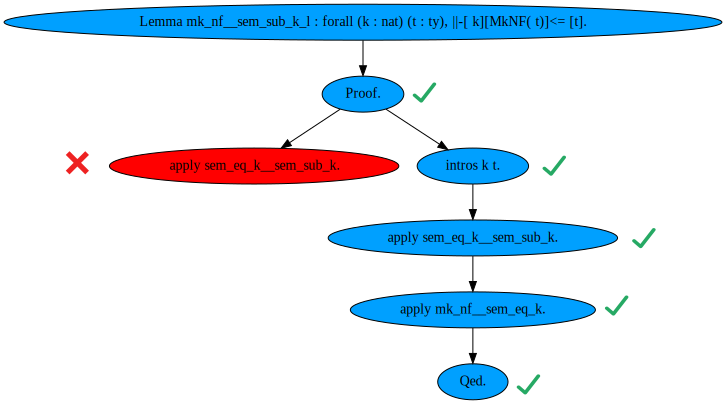
\includegraphics[width=0.70\textwidth]{maintenance/fig/example-graph.png}
  \caption{An example search tree, generated from the collected data
    by \toolname. It shows the user attempting to apply a lemma, which
    fails until they first run the \lstinline{intros} tactic.}
  \label{fig:search-tree}
\end{figure*}

\Cref{fig:tactics-table} shows the counts for each tactic
(regardless of arguments) in the 70 successful interactive proof subsessions.
%From this table, we can see that the
The distribution of tactics run was top-heavy; over 50\% of the tactics
invoked were either \lstinline{apply}, \lstinline{intros},
\lstinline{destruct}, \lstinline{rewrite}, \lstinline{exists}, \
\lstinline{unfold}, or \lstinline{simpl}.
The \lstinline{apply} tactic had a significant lead over other tactics
in invocations, but invocations of \lstinline{destruct} ended in
failure or stepping above them nearly as many times as invocations
of \lstinline{apply} did.

This data indicates two takeaways for proof tooling:
Firstly,
\begin{displayquote}
  \textbf{Takeaway:}
  Tools may be able to focus on understanding the behavior of
  and suggesting just a small number of tactics,
  and still benefit.
\end{displayquote}
And second, since lemma and hypothesis application was the main driver of proofs,
\begin{displayquote}
  \textbf{Takeaway:}
  Assessing which lemmas and hypotheses are useful would be one of the main tasks of
  a tool which suggests tactics to the user.
\end{displayquote}
The machine learning tool ML4PG~\cite{Komendantskaya2012} for Coq
already offers promising developments in this direction by understanding
and providing hints about similar lemmas,
as does the proof automation tool CoqHammer~\cite{coqhammer};
similar functionality may help
improve the performance of tools that suggest tactics.

\subsection{Fixing Proofs by Fixing Tactics}
\label{sec:fixes}

%While the raw cancellation numbers are useful, they do not give a
The raw cancellation numbers do not give a
broader context to each cancellation, namely what tactic it was
cancelled in favor of. To address this, we built a search
graph and analyzed the tactic attempts at each branching node (see
\Cref{fig:search-tree}). Where there were more than 2 attempts, we
compared all non-final attempts to the final one separately.

In our 71 successful interactive proof subsessions, 96 tactics
were cancelled in favor of another tactic at the same state.
Of the 96 cancelled-tactic and final-tactic pairs: %, we found:
\begin{itemize}
\item 13 were semicolon clauses added after a tactic, like:
  \begin{lstlisting}
    destruct w. $\to$ destruct w; reflexivity.
  \end{lstlisting}
\item 4 were semicolon clauses removed from the end of a tactic, like:
  \begin{lstlisting}
    intros; reflexivity. $\to$ intros.
  \end{lstlisting}
\item 31 were the same tactic with modified arguments, like:
  \begin{lstlisting}
    intros k X t. $\to$ intros k X t Hfresh.
  \end{lstlisting}
\item 5 were similar, but a \lstinline{Search} or \lstinline{Check} command was first run
  before replacing the tactic, like:
  \begin{lstlisting}
    apply IdSetFacts.remove_3. $\to$ 
    Check IdSetFacts.remove_3. 
    apply IdSetFacts.remove_3 with Y.
  \end{lstlisting}
\item 43 changes did not fall into this categorization.
\end{itemize}

The proofs shown were complex, and users often made nontrivial
changes to attempted tactics, so not all changes could be
easily categorized or analyzed. However, over half of the changes
present could be categorized into simple changes, and potentially
synthesized by automated tools.

This data also shows us that for a large proportion of tactics, users
could correctly pick the tactic to invoke, even when they made
mistakes in its arguments. In addition, fixing these arguments took both
on average and in the worst case longer than fixing other kinds
of mistakes. Accordingly,
\begin{displayquote}
  \textbf{Takeaway:}
  Automated tooling that suggests actions to take
  based on tactics that were recently stepped above or failed
  may focus on predicting new arguments for the attempted tactic.
\end{displayquote}

\section{Q2: Changes to Terms}
\label{sec:q2}

Q2 asked what kinds of changes proof
engineers make to programs and specifications, and whether those
changes reveal patterns amenable to automation.
This information may be useful to ensure tools for proof evolution
support the features that help proof engineers.

\paragraph{A2}
We found that while no single change was dominant across
all users, users made related changes within and across sessions.
Analysis of these changes revealed four patterns:

\begin{enumerate}
\item Incremental development of inductive types
\item Repetitive refactoring of identifiers
\item Repetitive repair of specifications
\item Interactive discovery of programs and specifications
\end{enumerate}

\paragraph{Methodology}
To answer this question, we wrote a script to visualize changes over 
time as diffs on Github (see Figure~\ref{fig:ex-diff}).
The script reconstructed the state of the file up to 
each cancellation within a session, then committed that to the 
public data repository.
When possible (see Section~\ref{sec:wish2}), it augmented
each commit with information on whether the cancellation was a failure
or the user stepping up in an IDE.

We then manually analyzed the diffs that this visualization produced to 
build a classification of changes (Section~\ref{sec:class}), 
then classify changes that we found (Section~\ref{sec:changes}).
We did this for each of the 362 interactive sessions and, when relevant,
across sessions as well.
Finally, we looked at clusters of common changes for patterns.
For each of the four patterns we found
(Sections~\ref{sec:pat1},~\ref{sec:pat2},~\ref{sec:pat3}, and~\ref{sec:pat4}),
we identified benchmarks (examples of the pattern in our data)
and lessons for automation.

\subsection{Building a Classification}
\label{sec:class}

After running the visualization script, we did a manual analysis of the diffs
in order to build a classification of changes to Gallina terms.
This analysis was thorough in that it involved inspecting each
consecutive diff and, when relevant, diffs that spanned several commits
(when a user stepped up, changed something, and then later stepped back down)
or sessions (when a user modified the same file during two different sessions).
However, it did not necessarily capture all changes to terms;
Section~\ref{sec:wish2} discusses some of the challenges.

\paragraph{Classification}

We designed a classification that groups changes along three dimensions:

\begin{enumerate}
\item \textbf{Command}: vernacular command used to define the term in
                        which a subterm changed
\item \textbf{Operation}: how the subterm changed
\item \textbf{Location}: innermost subterm that changed
\end{enumerate}
with the following categories for \textbf{Operation}:

\begin{enumerate}
\item \textbf{Structure}:
\begin{enumerate}
\item \textbf{Add} or \textbf{Del}: add or delete information
\item \textbf{Mov}: move information
\end{enumerate}
\item \textbf{Content}:
\begin{enumerate}
\item \textbf{Pch} or \textbf{Uch}: patch or unpatch
\item \textbf{Cut} or \textbf{Uut}: cut or uncut
\item \textbf{Rpl}: replace
\end{enumerate}
\item \textbf{Syntax}:
\begin{enumerate}
\item \textbf{Rnm}: rename
\item \textbf{Qfy} or \textbf{Ufy}: qualify or unqualify
\end{enumerate}
\end{enumerate}
Changes listed together are inverse operations.
The \textbf{Structure} changes are straightforward.
Among the changes to \textbf{Content}, \textbf{Pch} is applying a function
to the old term to get a new term, \textbf{Cut} is defining a new term
or let-binding and then referring to that term inside of an existing term,
and \textbf{Rpl} is replacing contents in any other way.
Among the \textbf{Syntax} changes, \textbf{Qfy} is
qualifying a constant after changing an import.

For \textbf{Structure} changes, there are five \textbf{Location}s:

\begin{enumerate}
\item \textbf{Hyp}: hypothesis of anything that can take arguments
\item \textbf{Arg}: argument in an application
\item \textbf{Ctr}: constructor of an inductive type
\item \textbf{Cas}: case of a match statement
\item \textbf{Bod}: body of anything that can take arguments
\end{enumerate}

For \textbf{Content} changes, there are an additional two:

\begin{enumerate}
\setcounter{enumi}{5}
\item \textbf{Fun}: function in an application
\item \textbf{Typ}: type annotation
\end{enumerate}

For \textbf{Syntax} changes, there are only three:

\begin{enumerate}
\item \textbf{Bnd}: binding in the local environment
\item \textbf{Idn}: identifier in the global environment
\item \textbf{Con}: constant
\end{enumerate}

\paragraph{Design Considerations}

That classification that we designed considers changes only within
Gallina terms defined or stated using vernacular commands.
Since it is focused solely on changes to defined terms,
it does not consider other information like changes to vernacular commands,
hints, tactics, notations, scope annotations, inference information, or imports,
and it considers additions of new terms only in \textbf{Cut} changes.

In building this classification, we aimed to group
changes at a level of granularity narrow enough to inform the design of proof
engineering tools, but broad enough to capture patterns.
We suspect that within these categories, there are more granular
categories that can be useful for automation, like distinguishing among
hypotheses to set apart indices of inductive types, or classifying
a \textbf{Content} change as semantics-preserving.
We did not design a more granular classification because we did not
find it useful for describing our data.
%(we found no changes to indices of inductive types, for example).

\subsection{Classifying Changes}
\label{sec:changes}

Once we had designed this classification,
we used it to classify the changes that we had found.
We ignored intermediate changes that immediately failed to lex, parse, or type check.

\begin{figure*}
\small
\begin{tabular}{ |l|rrrr|l|l|l| }
\hline
     \textbf{User} &
     \multicolumn{4}{c|}{\textbf{Top Changes}} &
     \textbf{\# Changes} &
     \textbf{\# Interactive} &
     \textbf{Expertise}
\\
\hline
     \textbf{1} &
     \indpat{\textbf{Add} \textbf{Ctr} (23)} &
     \indpat{\textbf{Add} \textbf{Cas} (22)} &
     \refactorpat{\textbf{Qfy} \textbf{Con} \phantom{0}(6)} &
     &
     \phantom{0}69 &
     \phantom{0}10 &
     $\circ$ $\circ$ $\circ$
\\
%\hline
     \textbf{2} &
     \indpat{\textbf{Add} \textbf{Cas} \phantom{0}(4)} &
     &
     &
     &
     \phantom{0}10 &
     \phantom{00}3 &
     $\circ$ $\circ$ $\circ$ $\circ$
\\
%\hline
     \textbf{3} &
     \repairpat{\textbf{Pch} \textbf{Arg} (13)} &
     \pddpat{\textbf{Mov} \textbf{Arg} \phantom{0}(8)} &
     \textbf{Add} \textbf{Bod} \phantom{0}(7) &
     \textbf{Cut} \textbf{Arg} \phantom{0}(7) &
     \phantom{0}55 &
     101 &
     $\circ$ $\circ$ $\circ$ $\circ$ $\circ$
\\
%\hline
     \textbf{5} &
     \indpat{\textbf{Add} \textbf{Cas} (20)} &
     \indpat{\textbf{Add} \textbf{Ctr} (13)} &
     \indpat{\textbf{Add} \textbf{Hyp} (12)} &
     &
     \phantom{0}75 &
     \phantom{0}15 &
     $\circ$ $\circ$ $\circ$
\\
%\hline
     \textbf{7} &
     \refactorpat{\textbf{Rnm} \textbf{Idn} (42)} &
     \pddpat{\textbf{Mov} \textbf{Hyp} (18)} &
     \pddpat{\textbf{Add} \textbf{Hyp} (18)} &
     &
     151 &
     183 &
     $\circ$ $\circ$ $\circ$ $\circ$
\\
%\hline
     \textbf{8} &
     \repairpat{\textbf{Rpl} \textbf{Fun} (29)} &
     \pddpat{\textbf{Del} \textbf{Hyp} \phantom{0}(4)} &
     \pddpat{\textbf{Uch} \textbf{Arg} \phantom{0}(4)} &
     &
     \phantom{0}44 &
     \phantom{0}27 &
     $\circ$ $\circ$ $\circ$ $\circ$ $\circ$
\\
%\hline
     \textbf{10} &
     \pddpat{\textbf{Pch} \textbf{Arg} \phantom{0}(4)} &
     \textbf{Rpl} \textbf{Cas} \phantom{0}(3) &
     &
     &
     \phantom{0}15 &
     \phantom{0}15 &
     $\circ$ $\circ$ $\circ$
\\
%\hline
     \textbf{11} &
     \textbf{Pch} \textbf{Cas} \phantom{0}(3) &
     &
     &
     &
     \phantom{00}7 &
     \phantom{00}8 &
     $\circ$ $\circ$ $\circ$
\\
\hline
\end{tabular}
\caption{Top changes, by user.}
\label{tab:userchanges}
\end{figure*}
% TODO Talia: Check patterns in anything not highlighted
% TODO Talia: Check timestamps and integrate if interesting
% TODO!!! Check user 2 for some constructors.

\begin{figure*}
\begin{minipage}{0.41\textwidth}
\centering
\includegraphics[width=0.7\textwidth]{maintenance/fig/diffs1.png}
\end{minipage}
\hfill
\begin{minipage}{0.57\textwidth}
\centering
\includegraphics[width=0.7\textwidth]{maintenance/fig/diffs2.png}
\end{minipage}
\caption{A change to an inductive type (left) and corresponding change to a fixpoint (right) that User 5 made in Session 19.}
\label{fig:ex-diff}
\end{figure*}

Classifying changes revealed clusters of related changes.
Further inspection of those clusters revealed common development patterns.
Figure~\ref{tab:userchanges} lists, for each user, the top three changes
by \textbf{Operation} and \textbf{Location} 
(four if there was a tie, and ignoring changes that we found fewer than three times for the user),
the total number of changes that we found,
and the total number of  interactive sessions and self-rated expertise
for reference.
Changes for which more detailed inspection revealed patterns
are highlighted in corresponding colors:
\indpatt{blue} for incremental development,
\refactorpatt{orange} for refactoring, \repairpatt{pink} for
repair, and \pddpatt{grey} for discovery.

The remainder of this section discusses these patterns, complete
with an example, benchmarks, and lessons for automation 
for each.
The benchmarks and lessons for automation are mainly for tool designers:
The benchmarks point to changes in specific sessions, the partial or 
complete automation of which would have helped our users.
The lessons for automation are natural directions for improvements
to proof engineering tools given the patterns we have observed.

The public data repository contains a complete list of the changes
that we classified, as well as a detailed walkthrough of each benchmark.

\subsubsection{Incremental Development of Inductive Types}
\label{sec:pat1}

The most common changes for Users 1 and 5 were adding cases to match statements
(\textbf{Add} \textbf{Cas}) and adding constructors to inductive types
(\textbf{Add} \textbf{Ctr}).
These changes corresponded to incremental development of inductive types,
followed by corresponding extensions to match statements of functions
that destruct over them, or to inductive types that depend
on or relate to them.
This pattern sometimes spanned multiple sessions.
While this pattern was most prevalent for Users 1 and 5, it was also
present for Users 2 and 7.

The diffs in Figure~\ref{fig:ex-diff} show an example change to
an inductive type, along with a corresponding change to a fixpoint.
The change on the left adds five constructors and moves one constructor down.
The change on the right adds five corresponding cases and moves one
corresponding case down.

\paragraph{Benchmark 1}

The example change from \Cref{fig:ex-diff} came from
User 5, Sessions 18, 19, 27, 33, and 35.
There, over the course of three weeks, the user incrementally developed the inductive type \lstinline{Term}
along with a record \lstinline{EpsilonLogic} and fixpoints
\lstinline{simplify} (later renamed to \lstinline{identity}) and \lstinline{free_vars}.

\paragraph{Benchmark 2}

In Sessions 37 and 41, over two days,
User 1 incrementally developed similar inductive types
\lstinline{ST} and \lstinline{GT}, as well as fixpoints
\lstinline{Gamma}, \lstinline{Alpha}, and \lstinline{eq} 
that referred to them.

\paragraph{Lessons for Automation}

Given that several users show this pattern,
this is one use case for which better automation may help.
Automation may help proof engineers adapt other inductive types,
match statements, and proofs after extending inductive types
with new constructors.
We are not aware of any work on adapting related inductive types and 
match statements.
There is some work on adapting proof obligations to new
constructors~\cite{Boite2004},
and a proposed algorithm for generating proofs that satisfy those
obligations~\cite{Mulhern06proofweaving}, but nothing that exists for
a current version of Coq.

\begin{displayquote}
  \textbf{Takeaway}:
  Proof engineers could benefit from automation to help update proofs and definitions
  after adding constructors to inductive types.
  %% Up-to-date automation to help proof engineers adapt definitions
  %% and proofs after extending inductive types is an unaddressed
  %% opportunity make an impact.
\end{displayquote}

\subsubsection{Repetitive Refactoring of Identifiers}
\label{sec:pat2}

Users 1 and 7 showed a pattern of repetitive refactoring, through
qualifying constants after changing imports (\textbf{Qfy} \textbf{Con}),
and renaming identifiers (\textbf{Rnm} \textbf{Idn}) and the constants
that referred to them (\textbf{Rnm} \textbf{Con}), respectively.
This pattern sometimes spanned multiple sessions, and even simple refactorings
sometimes resulted in failures.

Figure~\ref{fig:refactor} shows an example renaming from the five
definitions at the top to the five definitions at the bottom.
The change renames the identifiers of these definitions to
follow the same convention, then makes the corresponding changes
to constants in the bodies of the last two definitions.  

\begin{figure}
  \includegraphics[width=0.19\textwidth]{maintenance/fig/refactor.png}
  \caption{Renaming of definitions in User 7, Session 93.}
  \label{fig:refactor}
\end{figure}

\paragraph{Benchmark 3}

The example from \Cref{fig:refactor} came from User 7, Session 93.
The definition of \lstinline{ty} failed, since User 7 had already
defined an inductive type with that name.
In response, User 7 renamed all of these
to follow the same convention.
This took four attempts, but only a few minutes.

\paragraph{Benchmark 4}

In Session 193, User 7 split the \lstinline{TVar} constructor
of the inductive type \lstinline{ty} into two constructors:
\lstinline{TBVar} and \lstinline{TFVar}. User 7 at the same time
split the fixpoint \lstinline{FV} into \lstinline{FFV} and
\lstinline{FBV}.
In Session 198, User 7 at the same time renamed the broken lemma
\lstinline{b_subst_var_eq} to \lstinline{b_subst_bvar_eq},
and substituted in \lstinline{TBVar} for \lstinline{TVar} in its body.

\paragraph{Benchmark 5}

User 1 imported the \lstinline{List} module in Session 37, commit 10.
After the import, \lstinline{In} referred to the list
membership predicate from the standard library, whereas previously it had
referred to \lstinline{Ensembles.In}. The 6 qualify constant changes that we
found for User 1 were changing \lstinline{In} to \lstinline{Ensembles.In}
inside of three existing definitions.
This took multiple tries per definition,
but only a few minutes in total.

\paragraph{Lessons for Automation}

Refactoring terms (rather than proof scripts) as in
RefactorAgda~\cite{wibergh2019} and Chick~\cite{robert2018}
would have helped our users, but few refactoring tools for
ITPs support this~\cite{PGL-045}, and neither of these are implemented
for Coq.
Supporting making similar changes throughout a program, like Chick does,
may be especially useful.
Semantics-aware refactoring support may take this even further:
A refactoring tool for Coq may, for example, determine that an import
shadows an identifier, compute what the identifier used to refer to,
and refactor appropriately.
Or, it may guide the user to rename terms that refer to other
recently renamed terms.
Both of these would have helped our users.

\begin{displayquote}
  \textbf{Takeaway}:
  Refactoring and renaming tools,
  similar to those available for programmers in languages like Java,
  could also help proof engineers,
  and could potentially be more powerful in ITPs.
%%   Proof refactoring tools should support term refactoring,
%% especially patterns of term refactoring that are informed by Coq's semantics.
\end{displayquote}

\iffalse
Hooking into the REPL, like \toolname does, may help refactoring tools
make these suggestions independently of the UI.
\fi

\subsubsection{Repetitive Repair of Specifications}
\label{sec:pat3}

The top changes that we found for Users 3 and 8 were 
patching arguments (\textbf{Pch} \textbf{Arg}) and replacing functions
(\textbf{Rpl} \textbf{Fun}), respectively.
These corresponded to a pattern of repetitive repair of specifications,
often over several sessions.
Sometimes these repairs were necessary in order for the specification to
type check or for existing tactics to succeed.
Sometimes, after repairing specifications, users also repaired their proofs.

\begin{figure}
  \includegraphics[width=0.47\textwidth]{maintenance/fig/patch.png}
  \caption{Patches to a lemma in User 3, Session 73.}
  \label{fig:patch}
\end{figure}

Figure~\ref{fig:patch} shows an example change patching the arguments
of a lemma. This change wraps two arguments into a single application
in three different hypotheses of a lemma.

\paragraph{Benchmark 6}

11 of the 13 patches to arguments that we found for User 3,
including the example in \Cref{fig:patch}, came from Session 73.
All of these changes similarly wrapped arguments into an application of
\lstinline{Val}.
We suspect that this was due to a change in the definition of \lstinline{absr},
but we were not able to confirm this since
the change in question occurred before the beginning of the study.
The user admitted or aborted the proofs of four of the five
changed lemmas.

\iffalse
For the same reason, we were not able to determine with certainty
that the changes to proofs in that session were corresponding
repairs to match the new specification.
\fi

\paragraph{Benchmark 7}

28 of the 29 replace function changes that we found for User 8
were changes from \lstinline{=} to \lstinline{==} over
the course of about a week in Sessions
2, 14, 37, 40, 65, 79, 108, 125, and 160.
The corresponding proof attempts suggest that while these terms were well-founded with \lstinline{=}, the changes to use \lstinline{==}
may have been necessary to make progress in proofs
using certain tactics.
Sometimes, after making these changes, User 8 also fixed tactics
that had worked before.

\paragraph{Lessons for Automation}

Automation may help with these sorts of repairs to theorems
and proofs. The proof repair tool \textsc{PUMPKIN PATCH} already handles some
repairs to proofs after changes to both
\textbf{Content}~\cite{Ringer2018} and \textbf{Structure}~\cite{Ringer2019}, but has support for repairing the theorem statement itself only in
the latter case, and only for a specific class of changes to inductive types.
These changes provide examples where changing the theorem type is also
desirable, and may make good benchmarks for further development
to support this.

\begin{displayquote}
  \textbf{Takeaway}:
  Proof repair tools should repair programs and specifications,
  not just proofs.
\end{displayquote}

\subsubsection{Interactive Discovery of Programs and Specifications}
\label{sec:pat4}

In Q1 (Section~\ref{sec:q1}), we found that users most often fixed
proofs by stepping up outside of proofs and changing other things.
Our observations from Q2 are consistent with this,
and give some insight into the details.
Changes from Users 3, 7, 8, and 10 all revealed a pattern of interactive
discovery of programs and specifications:
In some cases, these users discovered bugs in their programs during a
proof attempt or test.
In other cases, these users discovered that their specifications were
incorrect, too weak, or difficult to work with.
Users sometimes assigned temporary names to lemmas or theorems,
then renamed them only after finalizing their types.
Even experts made mistakes in programs and theorem statements
(perhaps they were the ones catching them most effectively).

\begin{figure}
  \includegraphics[width=0.35\textwidth]{maintenance/fig/bad.png}
  \caption{A partial attempt at proving and later correction to an incorrect theorem from User 3, Session 11377 (tactic formatting is not preserved in the data
that \toolname receives).}
  \label{fig:bad}
\end{figure}

Figure~\ref{fig:bad} shows an example of catching a bug in a specification
during an attempted proof attempt. The theorem
before the change is impossible (let \lstinline{m} be \lstinline{3} 
and \lstinline{n} be \lstinline{1}).
After attempting to prove it and reaching this goal:

\begin{lstlisting}
  m : nat
  --------
  0 = m
\end{lstlisting}
the user steps up and fixes the theorem statement by replacing an argument
(\textbf{Rpl} \textbf{Arg}), then later finishes the proof.

\paragraph{Benchmark 8}

The change from \Cref{fig:bad} can be found in User 3, Session 11377.
The same session contains changes to the same theorem by
moving arguments (\textbf{Mov} \textbf{Arg}).
The user succeeded at the proof after about three minutes.
%All of the changes moving arguments that we found for User 3
%corresponded to interactive discovery of fixpoints and theorems.

\paragraph{Benchmark 9}

In Session 13, commit 11, User 10 patched a case (\textbf{Pch} \textbf{Cas})
of a fixpoint \lstinline{fib'} after testing.
This took the user about thirty seconds.
The fixpoint \lstinline{fib'} itself may have been used to 
test a different function.

\paragraph{Benchmark 10}

User 7 mainly demonstrated this pattern through
adding and moving hypotheses (\textbf{Add} and \textbf{Mov} \textbf{Hyp}).
The latter most often
corresponded to generalizing the inductive hypothesis 
after a partial proof attempt by swapping theorem hypotheses,
in some cases in order to induct over a different hypothesis 
altogether.
We found such changes in Sessions 19, 56, 93, 94, 104, 110,
153, 159, and 176.
See, for example, \lstinline{match_ty__value_type_l} in Session 94,
commit 15.

\paragraph{Benchmark 11}

In Session 2, User 7 temporarily named a lemma
\lstinline{weird_trans}, then renamed it to \lstinline{sub_r_nf__trans}
by Session 10 after finalizing its type after several partial
proof attempts over the course of about a day and a half.

\paragraph{Lessons for Automation}

The effect of discovering bugs by attempting a proof accounts for some
of the benefits of verification~\cite{murraybp}.
It makes sense, then, to continue to build automation to support users
in finding and fixing those bugs.
One possible unexplored avenue for this is integrating repair tools
with QuickChick~\cite{Paraskevopoulou2015} for testing specifications,
or with the \lstinline{induct} tactic from FRAP~\cite{FRAPBook}
or the hypothesis renaming functionality from CoqPIE~\cite{Roe2016}
for simple generalization of inductive hypotheses.
Integrating tools for discovering lemma and theorem names~\cite{Aspinall2016b}
during the development process may help users who use temporary names.
Above all, repair is not just something that happens to stable proof
developments---change is everywhere in developing those programs and
proofs to begin with.

\begin{displayquote}
  \textbf{Takeaway}: Integrating tools for proof repair with tools
  for discovery and development of specifications
  is an unaddressed opportunity to support proof engineers.
\end{displayquote}
